\section{Web-Framework (H.L.)}

Für die Webseite selbst wurde das Web-Framework Angular \cite{angular} genutzt. Angular selbst ist ein TypeScript-basiertes Front-End-Webapplikationsframework, welches besonderen Wert auf mobile Platformen legt. Zusätzlich erlaubt es eine objektorierte Programmierung.  
Das Ziel der Webseite ist es unsere Daten übersichtlich und sinnvoll darzustellen. Dafür wurde ein Dashboard entwickelt, welches mehrere Filteroptionen bietet.


\subsection{Module}

In Angular erzeugt man einzelne Komponenten, die später als Modul auf der Webseite angezeigt werden können. Unsere erstellten Module unterteilen sich so:

\begin{itemize}
    \item App-routing Modul
    \item Dashboard Modul
    \item Map Modul
    \item Wettervorhersagen Modul
    \item Wasserstand/KPI Modul
    \item Info Modul
    \item Kontakt Modul
    \item API Modul
\end{itemize}

\begin{figure}[!htb]
 \centering
 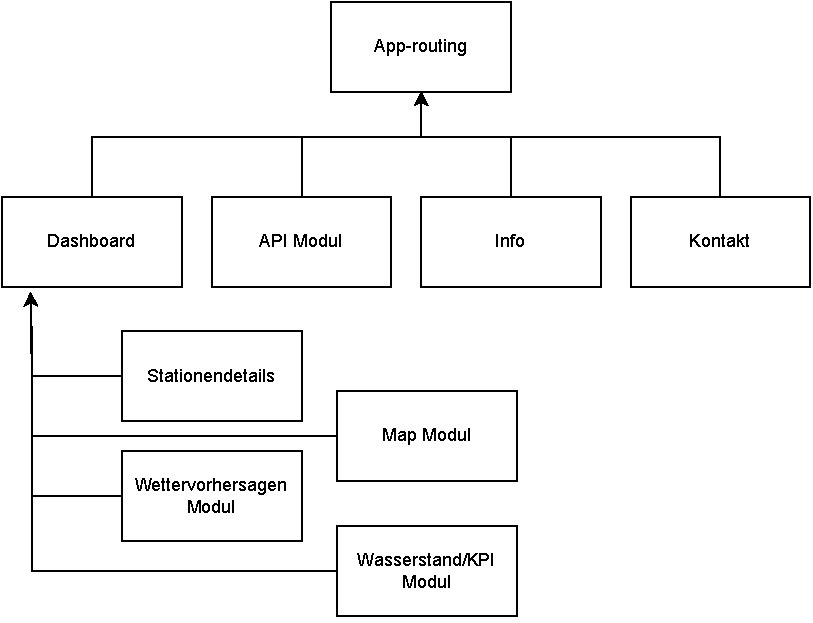
\includegraphics[width=10cm]{figures/Build.pdf}
 \caption{Bild des Aufbaus}
 \label{fig:Bild des Aufbaus}
\end{figure}

\newpage
\subsection{App-routing Modul}

Das App-routing Modul verwaltet die einzelnen Routen zu den jeweiligen Komponenten, um den Inhalt korrekt dazustellen und zu laden. Dafür haben wir auf die Angular-Router Bibliothek zurückgegriffen, die Methoden zur Verfügung stellt, um ein Routing zu realisieren. Von uns genutzte Klassen sind dabei das RouterModule und Routes. Dies ermöglicht uns eine dynamische Webapp Oberfläche, ohne die Seite neu zu laden bei einer Änderung des Inhalts.
\begin{figure}[!htb]
 \centering
 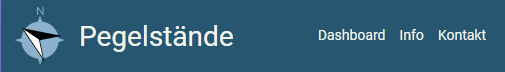
\includegraphics{figures/Navigation.PNG}
 \caption{Bild der Navigationleiste (Gestaucht)}
 \label{fig:Bild der Navigationleiste (Gestaucht)}
\end{figure}

\subsection{Dashboard Module}

Unser Dashboard Modul soll die in der Datenbank enthaltenen Daten visualisieren und verständlich erläutern. Dafür nutzen wir globale Filter, über die der Datenstand gewählt werden kann, das gemessene Attribut ausgesucht werden kann und die genauer betrachtete Station ausgewählt werden kann. Zusätzlich zeigen wir Informationen zum letzten Import aus der Datenbank, diese beinhalten den Datenstand und Anzahl der Stationen mit Daten. Bei der Visualisierung von dem Verlauf und den allgemeinen Informationen bietet ein Plotly-Linegraph einen übersichtlichen Einblick in den Verlauf der Daten. Für weitere Informationen geben wir den Namen, die zuständige Behörde, das Gewässer und den Kilometerstand an. Neben Plotly einer JavaScript Open-Source Graphing-Library, haben wir auch Angular Material genutzt, Material Design components for Angular, um graphische Komponenten wie Karten und Auswahlfelder darstellen zu können. Diese Komponenten sind auf Verlässlichkeit und Perfomance getestet.
\begin{figure}[!htb]
 \centering
 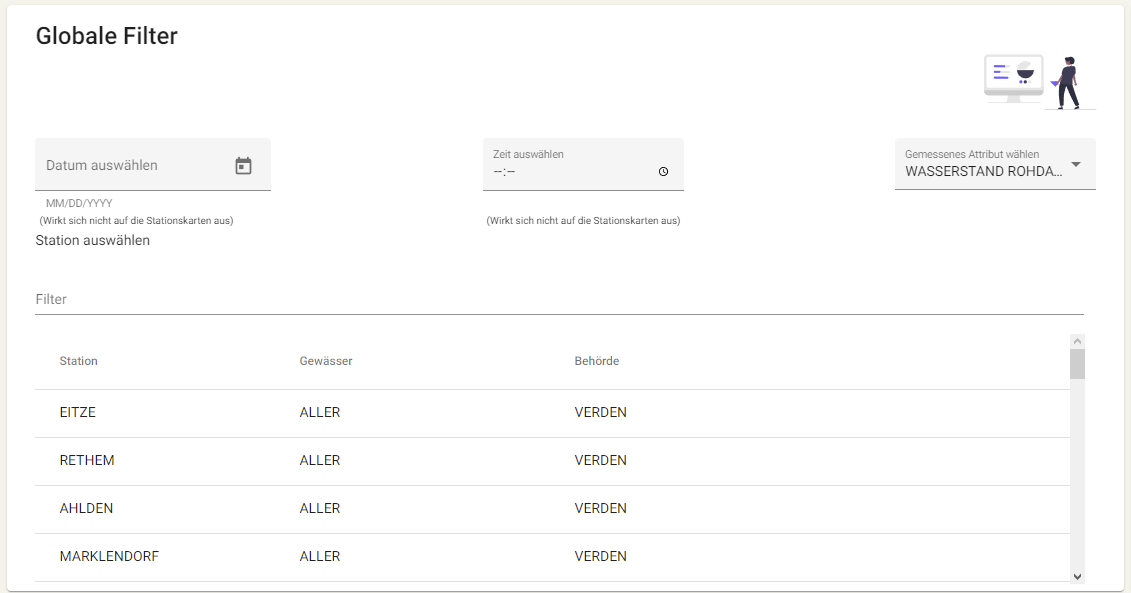
\includegraphics[width=12cm]{figures/Liste.PNG}
 \caption{Bild der Filteroptionen}
 \label{fig:Bild der Filteroptionen}
\end{figure}

\begin{figure}[!htb]
 \centering
 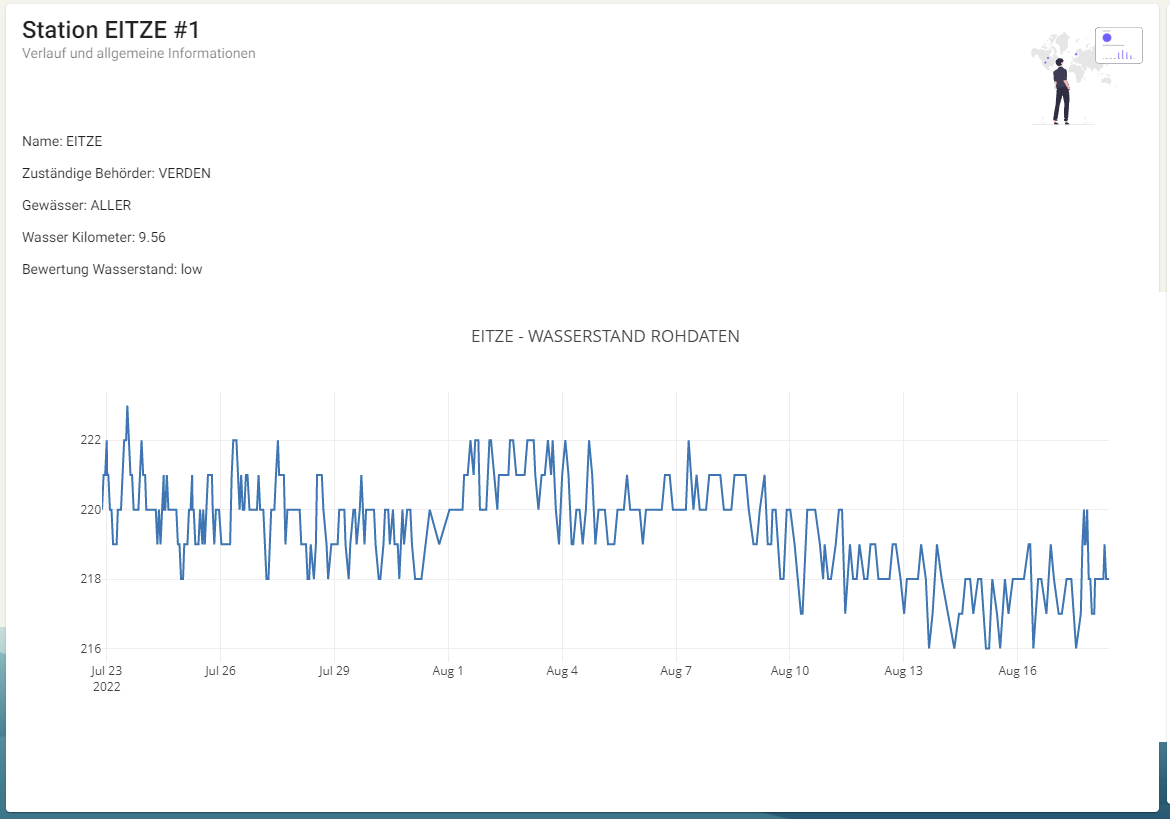
\includegraphics[width=12cm]{figures/Graph.PNG}
 \caption{Bild des Graphen}
 \label{fig:Bild des Graphen}
\end{figure}

\newpage
\subsection{Map Modul}

Um auch die Daten der Längen- und Breitengrade nutzen zu können haben wir eine Karte mit Markern integriert, die diese Standorte der einzelnen Stationen anzeigt. Plotly hat uns Kartenfunktionalitäten zur Verfügung gestellt. Für die Kartenteile haben wir OpenStreetMap verwendet, dieses Projekt stellt frei nutzbare Geodaten zur Verfügung (\url{https://www.openstreetmap.de}). Die einzelnen Marker öffnen ein Popup, welches den Namen der Station offenbart und die Informationen der Station aufruft. Zusätzlich zeigt es auch nur die Stationen an, von denen Daten mit dem passenden Attribut existieren. Die Marker selbst färben sich auch ein je nach dem, wie hoch die Werte sind. So wird ein Überblick über alle Stationen geben, hinsichtlich der aktuellen Lage. Dies hilft zu sehen, ob ein Extremwert nur an einer Station ist oder über mehrere Stationen zu erkennen ist. Dadurch können Trends und Veränderungen der Werte verfolgt werden.
\begin{figure}[!htb]
 \centering
 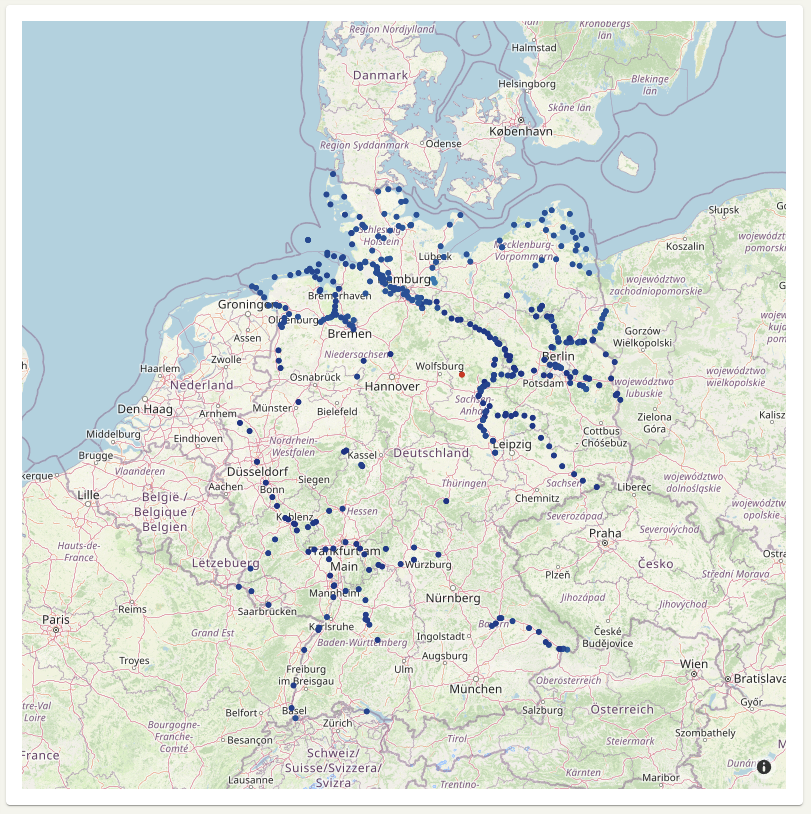
\includegraphics[width=8cm]{figures/Map.PNG}
 \caption{Bild der Karte}
 \label{fig:Bild der Karte}
\end{figure}

\newpage
\subsection{Wettervorhersagen Modul}

Dieses Modul gibt einem auch noch Auskunft darüber, wie das Wetter werden soll. Dazu wird die API des Deutschen Wetterdienst angesprochen, welche Meteorologische Wetterdaten im Rahmen des Open Data program veröffentlicht (\url{https://www.dwd.de/DE/leistungen/opendata/opendata.html}). Wir nutzen diese Chance um auch eine Verbindung zwischen vergangenen Daten aus unserer Datenbank und Prognosen zu schaffen. Dieser Ausblick auf zukünftige Wetterprognosen kann helfen die zukünftigen Daten zu schätzen.

\begin{figure}[!htb]
 \centering
 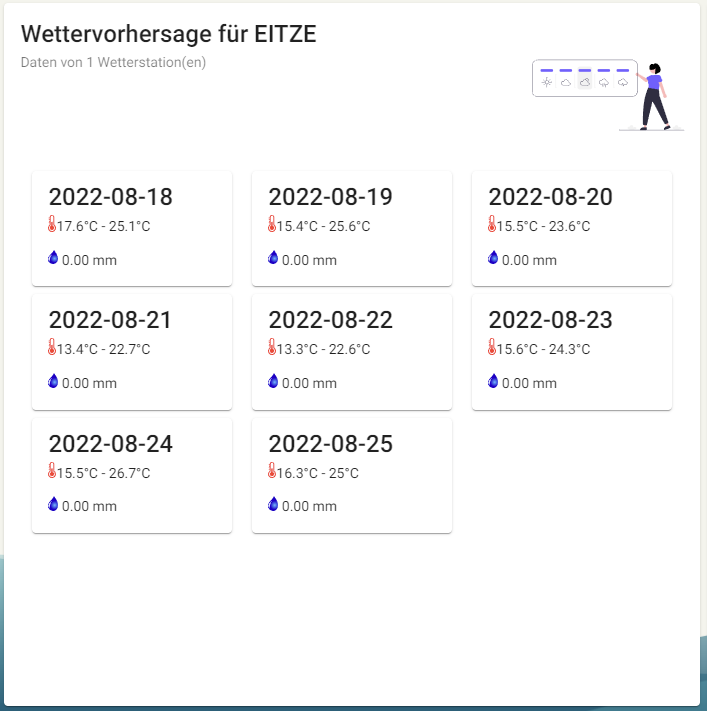
\includegraphics[width=10cm]{figures/Wettervorher.PNG}
 \caption{Bild der Wettervorhersage}
 \label{fig:Bild der Wettervorhersage}
\end{figure}
\newpage
\subsection{Wasserstand/KPI Modul}

Ein Messdiagramm wird genutzt um den Wasserstand darzustellen, wodurch der aktuelle Wert zwischen dem Minimum und dem Maximum sichbar wird. Zusätzlich wird auch die Veränderung zum vorherigen Wert gezeigt. Farbliche und symbolische Indikatoren werden auch genutzt, um dem User einen schnellen Eindruck zu vermitteln. 
\begin{figure}[!htb]
 \centering
 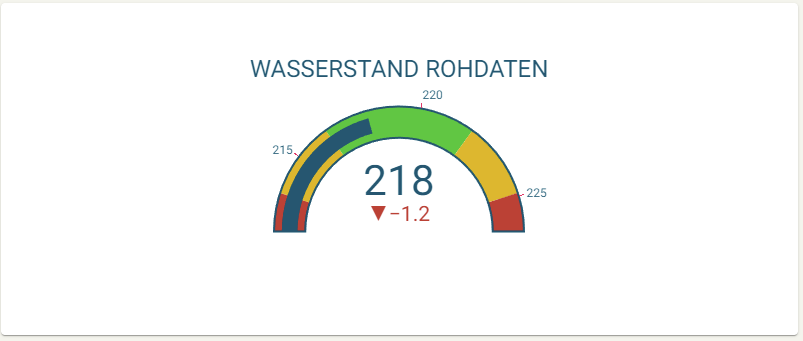
\includegraphics[width=13cm]{figures/OnlyGauge.PNG}
 \caption{Bild der Wasserstandsanzeige }
 \label{fig:Bild der Wasserstandsanzeige }
\end{figure}

\begin{figure}[!htb]
    \centering
    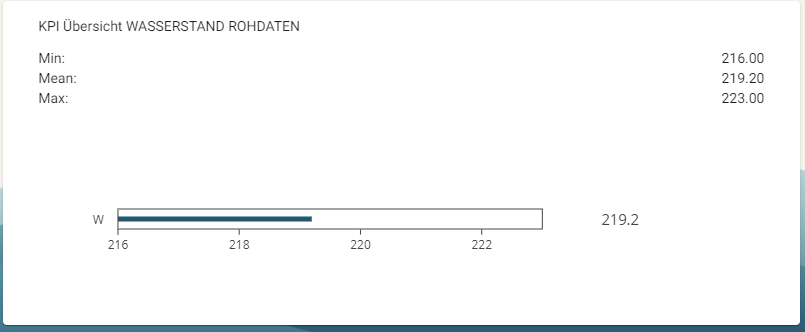
\includegraphics[width=13cm]{figures/KPI.PNG}
    \caption{Bild der KPI Anzeige}
    \label{fig:Bild der KPI Anzeige}
   \end{figure}

\newpage
\subsection{Info Modul}

Hier werden nur Informationen erläutert in welchem Rahmen dieses Projekt entstandt, wer daran beteiligt ist und was die Funktionalität umfassen soll.

\begin{figure}[!htb]
 \centering
 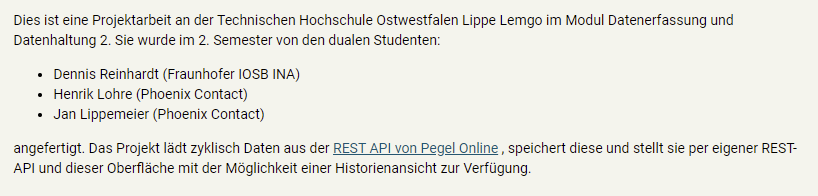
\includegraphics[width=15cm]{figures/Info.PNG}
 \caption{Bild der Info}
 \label{fig:Bild der Info}
\end{figure}

\subsection{Kontakt Modul}

Hier wurden ein paar Infokarten zu den Entwicklern eingebaut und die zusätzlich die Aufgabeneinteilung abbilden sollen.

\begin{figure}[!htb]
 \centering
 
\includegraphics[width=13cm]{figures/Kontakt.PNG}
 \caption{Bild der Kontakte}
 \label{fig:Bild der Kontakte}
\end{figure}

\newpage
\subsection{API Modul}

Für die Daten der Datenbank wurde eine REST-API programmiert, die uns verschiedene Routen zur Verfügung stellt. In der Angular Webapp selbst haben einen Service geschaffen der uns Funktionen und passende Interfaces bietet. Jedes Modul kann diese Methoden importieren und nutzen, sodass es für uns einfacher ist zentral Änderungen vorzunehmen. Angular unterscheidet zwischen Komponenten und Services, um die Modularität zu erhöhen und die Wiederverwendbarkeit.
Eine Komponente sollte Services für Aufgaben verwenden, die keine Anwendungslogik beinhalten. Services eignen sich für Aufgaben wie das Abrufen von Daten vom Server oder die Validierung von Benutzereingaben.

~\\
\begin{lstlisting}[language={JavaScript}, caption={Beispiel: DbContext eines Interfaces}, captionpos=b, label={Script}]
    export interface Station {
        AGENCY_NAME: string;
        IDNR: number;
        LATITUDE: number;
        LONGITUDE: number;
        LONGNAME: string;
        SHORTNAME: string;
        WATER: string;
        WATER_KM: number;
      }
\end{lstlisting}~\\